\subsection{Joining}
To join such an overlay, peers need to contact an entry point, also referred to as rendezvous point or \gls{signal-server} \cite{TODO}.
Peers need to discard their signal server connection after having entered the network, i.e. having acquired enough connections to other peers, to reduce the bottleneck–effect these entry points have on the system.
However, to allow new peers to join, entry points need to maintain at least one permanent contact to the network. This is ensured by so called \glspl{router} that keep a persistent connection to the signal and are thoroughly integrated into the mesh.

The joining procedure is started by the \newbieRole role inherent to new clients. The \newbieRole role seeks to connect to one of its pre–configured signal server addresses.
Upon connection, it sends an \introduction message to the signal, letting it know that it is looking for a cluster. The signal responds with two messages:
\begin{enumerate}
    \item a \roleUpdate that relieves the client from its \newbieRole role and promotes it to the \peerRole role
    \item a \peerUpdate that tells the \newbieRole the address of a \gls{router} to which it should connect.
\end{enumerate}
The new peer then adds the router address from the \peerUpdate to its local peer table, remembering that it is reachable via the connection to the signal.
It also switches its \newbieRole role for the \peerRole role and its connection acquisition mechanism, as described in \ref{TODO}, kicks in. It starts a connection negotiation process with the router. If the router has capacity to directly connect to the new peer, it will do so, otherwise it will name alternative peers to connect to.

In summary, there are three distinct scenarios, that can occur when a new peer enters the network: 1) the signal has no knowledge of a cluster and creates a new one 2) the signal can forward the new peer to a \routerRole peer which can directly accept it 3) the \routerRole peer has no capacity to adopt the new peer and forwards it deeper into the cluster.

\paragraph{Cluster Genesis}
\vref{fig:genesis} shows the genesis scenario with a newbie peer \alice approaching a signal server, conveniently named \signal. After the \introduction, \alice receives a \peerUpdate only containing the \signal itself and a \roleUpdate that promotes her to \peerRole and \routerRole roles. Alice changes updates her roles accordingly, adds the \signal to her peer table and begins with her first \routerRole duty: sending \alive messages to the \signal.

\paragraph{Direct Joining}
\vref{fig:peer-redirect} illustrates the subsequent scenario, where a second peer named \bob enters the network. As an \introduction response, \bob receives a \roleUpdate that promotes him to only the \peerRole and a \peerUpdate that now also includes the address of \routerRole \alice. As a \peerRole without the \routerRole role, \bob now strives to connect to \alice and to abandon the \signal. Steps 4 through 5 show the \connectionNegotiation, that is relayed by the \signal. After the connection to \alice is established, \bob disconnects from \signal and both peers start exchanging \peerUpdate messages periodically.

\paragraph{Redirected Joining}
\vref{fig:peer-redirect} illustrates the most complex peer–joining scenario. It assumes, \alice has reached its connection limit \ref{TODO} and cannot connect to the new peer named \zoe. Step \TODO{insert step number after figure has been updated with REJECT message} shows \alice responding to the connection offer from \zoe with a \rejection and a \peerUpdate. The \rejection lets \zoe know, that \alice is unable or unwilling to connect, but the \peerUpdate gives a set of alternative peers to try. \zoe picks \bob and sends a \connectionNegotiation which now has to be relayed through \signal and \alice. As \bob can connect to \zoe, she can end the \signal connection and start exchanging \peerUpdate messages with \bob.

TODO:
- Make arrow round 
- remove dots after message no
- 2b should be 3
\begin{figure}
\centering
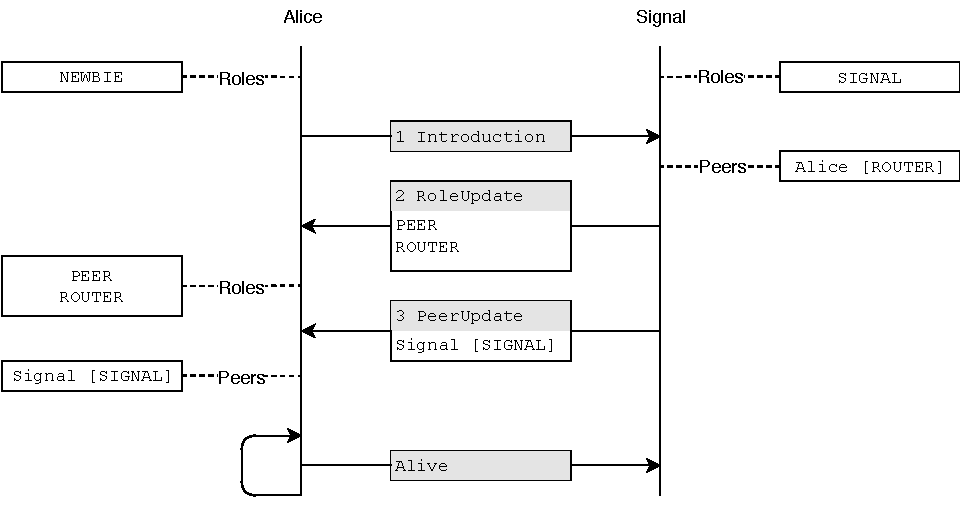
\includegraphics[width=1\textwidth]{graphics/design/genesis.pdf}
\caption{Cluster Genesis: Alice starts a new cluster and becomes its router.}
\label{fig:genesis}
\end{figure}

TODO:
- remove loop arrow at alice's peer update
- make alice send alive to signal
\begin{figure}
\centering
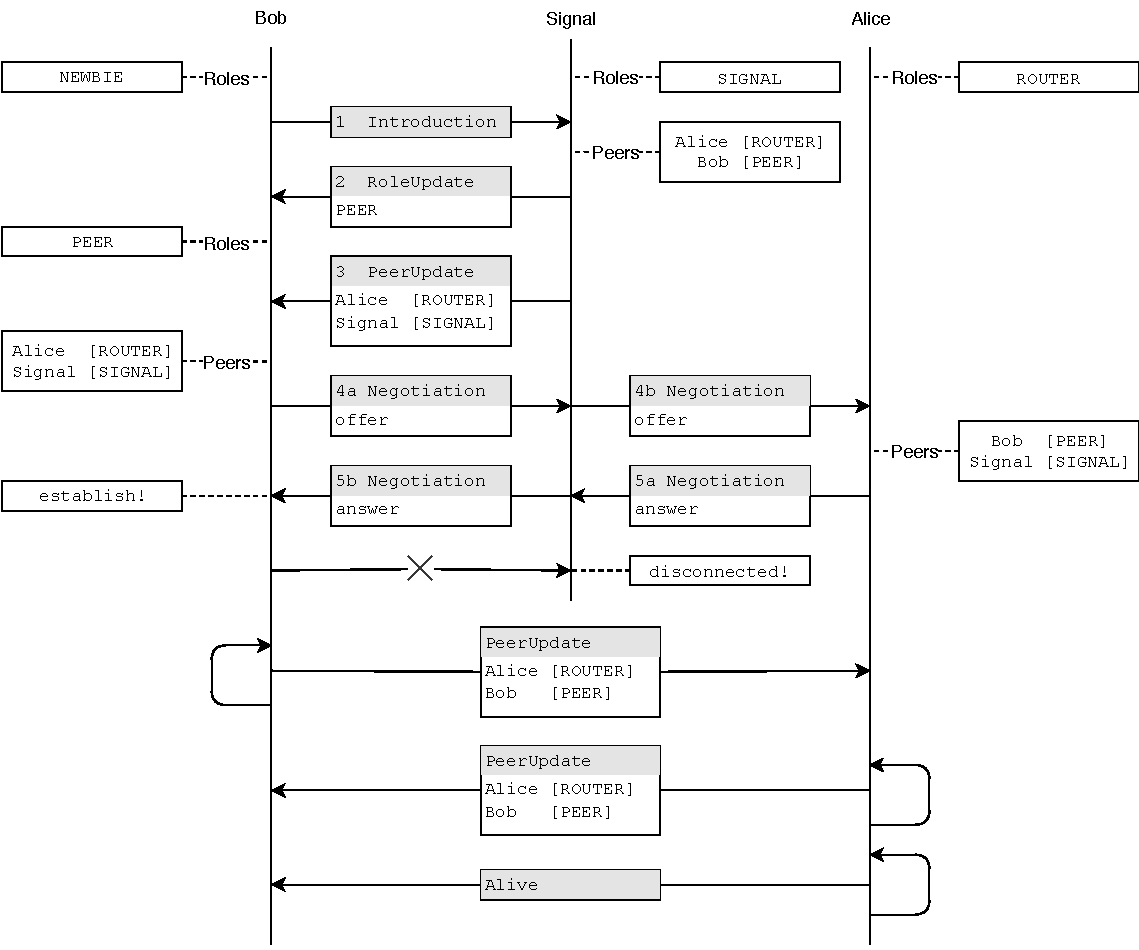
\includegraphics[width=1\textwidth]{graphics/design/peer-join.pdf}
\caption{Direct Joining: Bob joins Alice's cluster and can directly connect to her.}
\label{fig:peer-join}
\end{figure}


TODO:
- Put REJECT message in peer-redirect!
- remove alice alive flow, thats too much
\begin{figure}
\centering
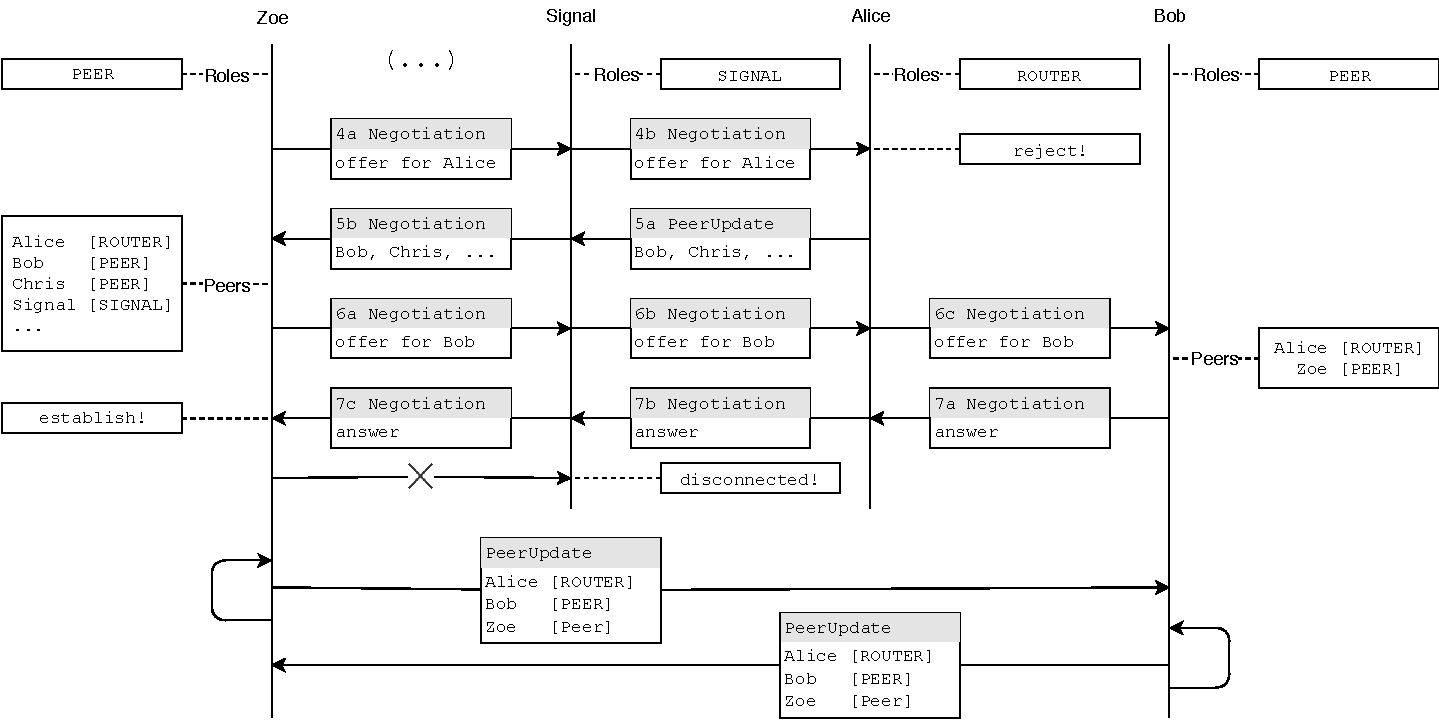
\includegraphics[width=1\textwidth]{graphics/design/join-redirect.pdf}
\caption{Redirected Joining: Alice has no capacity for Zoe and redirects to Bob.}
\label{fig:peer-redirect}
\end{figure}
